\documentclass[12pt,a4paper]{article}
\usepackage[utf8x]{inputenc}
\usepackage[english]{babel}
\usepackage{amsmath}
\usepackage{amsfonts}
\usepackage{minted}
\usepackage{amssymb}
\usepackage{graphicx}
\usepackage{lmodern}
\usepackage{graphicx}
\usepackage{flafter}
\usepackage{placeins}
\setlength{\parindent}{0cm}
%\usepackage[left=2cm,right=2cm,top=2cm,bottom=2cm]{geometry}
\author{Torje Hoås Digernes \& Einar Johan Trøan Sømåen}
\setlength{\parindent}{0cm}
\setlength{\parskip}{4pt}
\title{Problem set 6 - Shared memory computing and distributed memory computing. }
\begin{document}
\maketitle
\section{Introduciton}

\section{Solution strategies}
Given that we have a supercomputer at our hands we could be tempted to just
throw processing power on the problem until it disappears, but a simple solver
based on Elementary linear algebra would be very slow compared to other
solutions. A solver using gaussian elimination or LU-factorisation would have a
vector of unknowns being \emph{n}$^2$ long and require \emph{n}$^6$ floating
point operations. Given that each unknown only depends on its neighbours we have
a banded matrix and can shave off \emph{n}$^2$ and achieve the same result in
\emph{n}$^4$. 

Using properties that is in our stencil, our discretisation of the Laplace
operator, is itself transposed so we can use a three-point stencil: T, $\mathrm{PU}=\mathrm{TU+UT}$, which is
the same as we use in two dimensions, both ways, just swapping what side we
multiply with, then diagonalising T, putting us at \emph{n}$3$ floating point
operations. A further improvement on this method can be done replacing a vector
matrix product with a Fast sine transform, a transpose and a fast inverse sine
transform landing us at $\log(n)\cdot n^2$. We are not attempting to further
explain as we did not quite understand the diagonalisation part. 
	

\section{The program}
\subsection{Components of a solution}
Our program consists of three components that come together to produce a results to
the problem at hand, a matrix that holds the actual data, and some necessary metadata,
like row/column-count, a transpose-function for this matrix, that utilizes MPI for communication,
and finally the provided (inverse) fast sine transform-functions.

\subsubsection{The matrix}
We can set the matrix as the minimum memory we need as we do not attempt to
compress the information. The matrix is square and this results in it using
\emph{n} times the space a variable occupies. After finalising we saw that we
should have linked our struct directly to the MPI session as it never is used
without it and that would make the code somewhat more neat. 

\subsubsection{MPI and transposition}
MPI is only used to infer the local dimensions of the matrix and more directly
to do the communication during the transpose operation. We use what we consider
the minimum practical space required for this, auxillary memory being the same
size as the area where the matrix holds the data. To minimise the connections
needed we serialise the data before sending so that all data going from process
A and process B is in one sequence. After the data have been received in a
process it will do a transpose locally, since it must be done at one point and
after the transport step is the most convenient point to do it. 

Technically we could have managed with less auxiliary memory, but we believe this
would have resulted in longer running time, because we would need to do parts
of the transposition before we can continue the communication and thus add much more
complexity. 

\subsubsection{fast sine transform and inverse }
As the fortran file was not quite readable for us, we neatly wrapped up the
\texttt{fst\_()} and \texttt{fstinv\_()} functions in functions which allocates the
auxillary memory needed and dispatches the function which does the math. These
wrappers are trivially parallelisable using \emph{openMP}. 

\subsection{Putting it all together} 
By looking at the original program and figuring out what each part did we
mapped that to what we had implemented and put it together the same way, just
using our parallelised versions. The result looks more or less like this list,
except for timers that we included. 

\begin{itemize}
\item Initialise matrix
\item Initialise the eigenvalue vector to our operator
\item apply the fast sine transform on the matrix
\item transpose matrix
\item apply the fast inverse sine transform
\item divide the matrix elements by the eigenvalues of the operator ()
\item sine transform
\item transpose matrix
\item inverse sine transform to get the answer
\end{itemize}

\section{Errors}
Subsituting the formula in place of $f$ and comparing the result with the analytical answer yields us a difference we can compare to the expected convergence of the method. Table \ref{tab:relerr} shows that we have the convergence that we were after. To achieve this only the populate function and minus/campare funtion needed to be changed. As the bounds and edge conditions were left unchanged nothing more needed to be changed.  

\begin{table}[t]
\caption{\label{tab:relerr}Error in the differents resolutions lining up where we expect them to be. Multiplying the absolute error with the relative error correction, which matches a quadratic convergence in error, below gives near identical results for all resolutions. The function that were set in were -5 $\pi \sin(\pi x ) \sin(2\pi y)$ and it was compared to $\sin(\pi x ) \sin(2\pi y)$. }

{\footnotesize
\begin{tabular}{|c|c|c|c|c|c|c|}
\hline 
 &  2048 & 1024 & 512 & 256 & 128 & 64 \\ 
\hline 
abs. error &6.6671e-07  & 2.6668e-06 &  1.0667e-05  & 4.2670e-05 &  1.7069e-04 &  6.8297e-04\\
\hline 
rel. correction  & 1024 &   256   &  64   &  16  &    4   &   1\\
\hline 
& 6.8271e-04 &  6.8271e-04 &  6.8272e-04 &  6.8273e-04 &  6.8278e-04  & 6.8297e-04\\
\hline 
\end{tabular}
}
\end{table} 


\section{Non-homogeneous Dirichelet boundary} 
We are going to hazard a guess that we can make a sloping surface between the boundaries and deduct the corresponding value from the matrix, resulting in us returning to a homogeneous Dirichelet boundary equal to 0, apply this solution to problem, and afterwards add the surface again. 

\section{Extension in both directions}
As the $h$ is bound to the steplength, changing the total length from 1 to $L_x$ and $L_y$ changes how we compute it, we would seemingly be getting to $h$s, $h_y$ and $h_x$. We do also believe that this would have an effect on the eigenvalue vector, giving us 2, one for each direction. 
\section{Results}

\FloatBarrier
\begin{figure}[t]
  \centering
    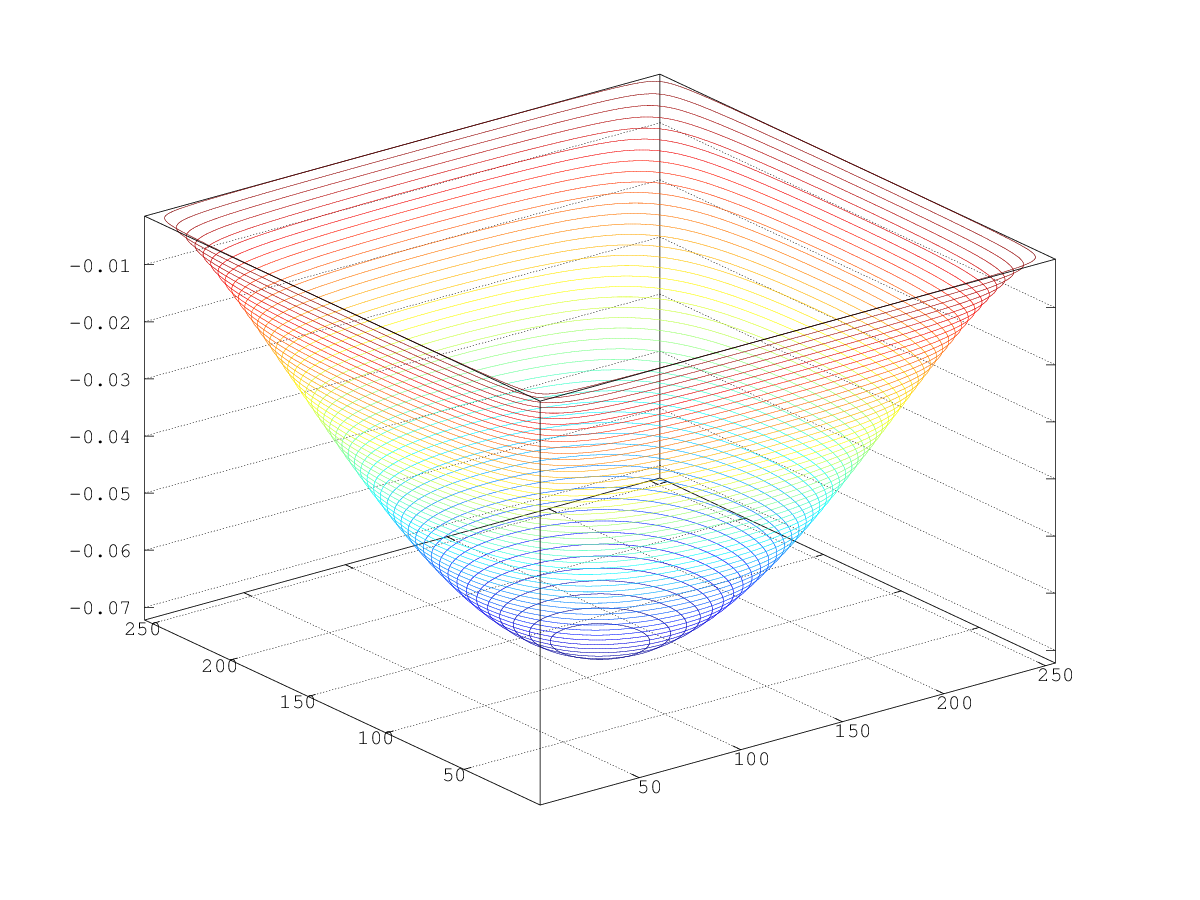
\includegraphics[width=0.7\textwidth]{datashit512flat_v2.png}
    \caption{$H^2$}
\end{figure}

\begin{figure}[t]
  \centering
    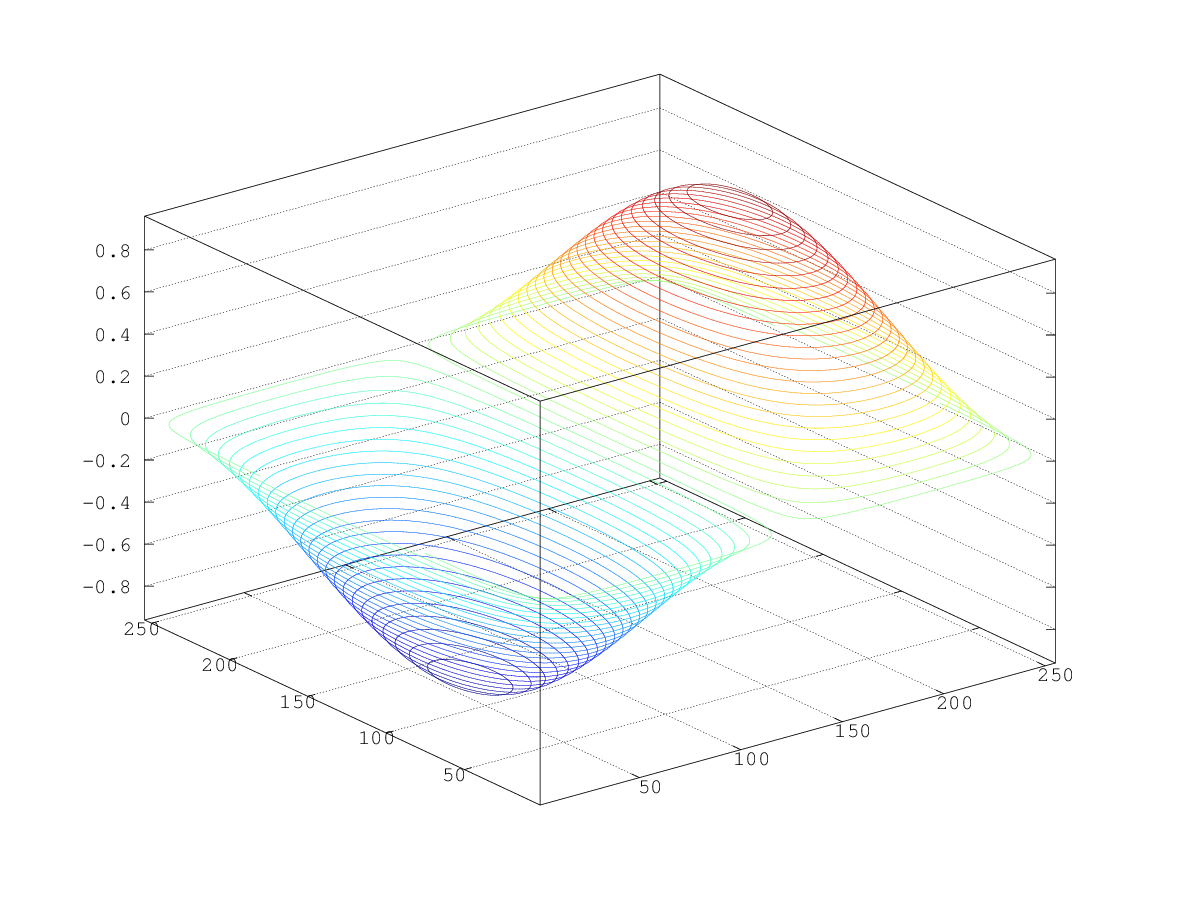
\includegraphics[width=0.7\textwidth]{datashit512sinpixsin2pix_v2.png}
    \caption{$(sin(\pi*x)\cdot sin(2\pi*y))\cdot 5\pi^2$}
\end{figure}
\FloatBarrier
We did some testing with various problem sizes to see how fast our program ran, then we
extrapolated the expected run time by using:
\begin{align}
k &= 
    \dfrac{n_{0}^2*\log{n_{0}}}{t}
\end{align}
\begin{align}    
t_{n} &= \dfrac
        {n^2\cdot\log{n}}
        {k} 
\end{align}

\begin{figure}[t]
  \centering
    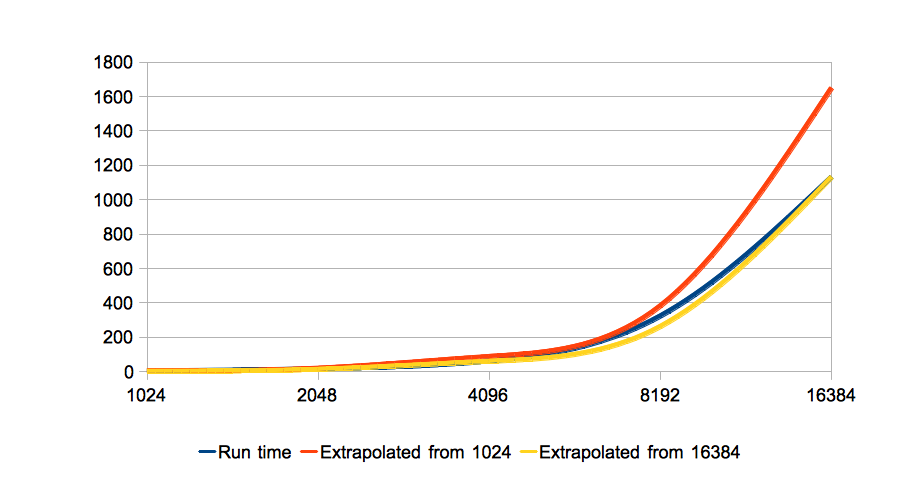
\includegraphics[width=0.8\textwidth]{speed_over_size_3.png}
    \caption{Run time for various problem sizes, compared to their extrapolation}
    \label{runsize}
\end{figure}

To show a $n^2\cdot$log n extrapolation from the actual run time, as shown in figure \ref{runsize}, where we did an extrapolation from the run time of a problem set of size 1024 and up, and a similar extrapolation from the run time of a problem set of size 16 384. This shows that our runtime scales within the expected values, although the extrapolation looks closer when basing it on 16 384 than when basing it on 1024. This is partially because the smaller problem sets fit better into cache, but also because the actual run time dominates less than the constant-factors at these sizes.

We also did a comparison with regards to how our program scales with the amount of processes it is run with,
as shown in figure \ref{numprocs}, our run time does indeed go down, with an odd increase in speed between 6 processes and 9 processes.
\begin{figure}[t]
  \centering
    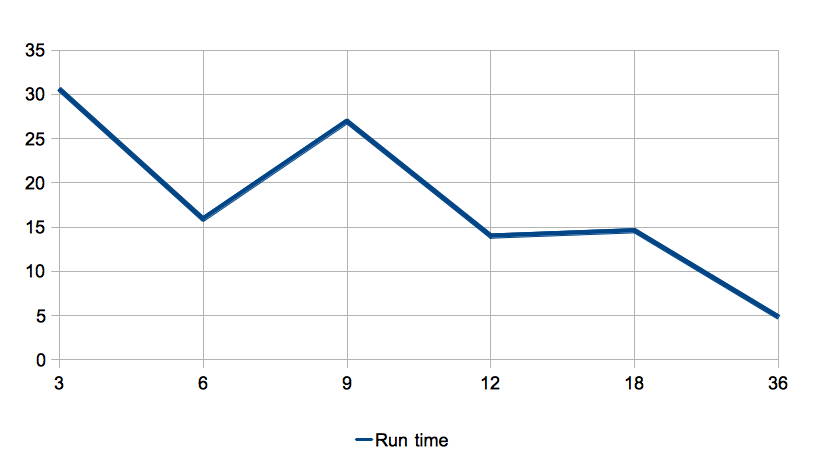
\includegraphics[width=0.8\textwidth]{run_time_over_np.png}
    \caption{Run time for problem size 4096 with varying process-amount}
    \label{numprocs}
\end{figure}

\FloatBarrier
\section{Utilities, Compilers and Hardware}

\subsection{Libraries}
Our program needs to be linked against the following libraries
\begin{itemize}
    \item{\texttt{libmpi}}  -  to get MPI-functionality
    \item{\texttt{libm}}  -  to get the necessary math-functionality.
\end{itemize}

\subsection{Compilers}
On Kongull we used the following compilers to compile our program:
\begin{itemize}
    \item{\texttt{GCC 4.7.0}}
    \item{\texttt{GFortran 4.7.0}}
\end{itemize}

Both of which had to be activated explicitly with \texttt{module load gcc/4.7.0}.

Locally we also did some testing, using these compiler-versions, with all warnings enabled to make sure that our code was as well written and portable as possible:
\begin{itemize}
    \item{\texttt{GCC 4.7.2}}
    \item{\texttt{GCC 4.2.1 (Apple LLVM)}}
    \item{\texttt{Clang 3.0}}
    \item{\texttt{Clang Apple LLVM 4.2 (based on LLVM 3.2svn)}}
    \item{\texttt{Gfortran 4.5.4}}
    \item{\texttt{Gfortran 4.7.2}}
\end{itemize}

\subsection{Kongull}

The distributed memory computer we ran our program on is called Kongull, it consists of 93 compute nodes that each have the following specs:
\begin{itemize}
    \item 24/48 GiB RAM
    \item 2x6 Core AMD Opteron 2431, each with the following specs:
    \begin{itemize}
        \item 2.4 GHz
        \item 6 x 128 L1 Cache
        \item 6 x 512 KiB L2 Cache
        \item 6 MiB L3 Cache
    \end{itemize}
\end{itemize}

Each of these nodes has 2 CPUs, that share memory, thus we enjoy the combination of shared memory computing AND distributed memory while
running on this cluster.
\section{Discussion}

Our program seems to have some variance in it's runtime, timing the various processes show values
between 0.5 and 9 seconds, this stems from the fact that the processes are using blocking communication
for the transpose, so the slowest process will delay the faster processes at these points, effectively creating
2 bottlenecks in our runs (one for each of the matrix transposes).

Our program is dominated by the (inverse) fast-sine-transform-calls runtime-wise, which we have little possibility
to optimise any further. We also use a large amount of small functions to do the various tasks that are required to
set up and manage the matrix, however, none of these are close to any tight loops, and most of them will be optimised
by the compiler so that inlining this functionality would not create any further runtime-benefits, but instead make the
code base less manageable.

The decision to wrap the fortran-code into C-functions should also not have any effect on the runtime, for the same reason
explained above, the functions will be link-time-optimised afterwards anyhow.

\section{Appendix A: Transpose-source code}

\subsection{mpiMatrix\_transpose}
\inputminted{c}{transpose.c}
\subsection{mpiMatrix\_serialiseForSending}
\inputminted{c}{serialise.c}
\subsection{mpiMatrix\_deserialiseAfterReception}
\inputminted{c}{deserialise.c}
\end{document}
